\colorlet{maincolor}{niceblue} % Color section in blue
\section[Client]{Client mit Backbone.js}

\begin{frame}{Architektur}
  \begin{center}
    \only<1>{
  \tikzset{
    every label/.style={
      font=\scriptsize\color{white}\bfseries,,
      inner sep=2pt
    }
  }
}
\only<2>{
  \tikzset{
    every label/.style={
      font=\scriptsize\color{maincolor}\bfseries,
      inner sep=2pt
    },
  }
}

\begin{tikzpicture}[
    node/.style={
      draw=maincolor,
      thick,
      rectangle,
      rounded corners,
      minimum width=6em,
      minimum height=4ex,
      inner sep=0ex,
      fill=maincolor!18},
    shorten >=1pt,
    line/.style={
      thick,
      color=maincolor
    },
    xs/.style={every edge/.append style={
      transform canvas={xshift=#1}
    }},
    ys/.style={every edge/.append style={
      transform canvas={yshift=#1}
    }},
    node distance=2em and 5ex
  ]

  \node[node, label={[name=Router label]BACKBONE}] (Router) {Router};
  \node[node, below=of Router, label={[name=StateModel label]CUSTOM}] (StateModel) {StateModel};
  \node[node, node distance=3em and -5ex, below right=of StateModel,label={[name=Views label]BACKBONE}] (Views) {Views};
  \node[node, node distance=3em and -5ex, above right=of Views,label={[name=DOM label]JQUERY}] (DOM) {DOM};
  \node[inner sep=0pt,above=of DOM] (Browser) {\pgfimage[width=4em]{images/browser}};
  \node[node, right=of Views,label={[name=Templates label]UNDERSCORE}] (Templates) {Templates};
  \node[node, below=of Views,label={[name=Collections label]BACKBONE}] (Collections) {Collections};
  \node[node, right=of Collections, label={[name=Ajax label]JQUERY}] (Ajax) {Ajax};
  \node[right=of Ajax,text width=4em,align=center] (Server) {\pgfimage[width=4em]{images/server}\newline Server};
  \node[node, below=of Collections,label={[name=Models label]BACKBONE}] (Models) {Models};
  
  \draw[line]
    (Browser) edge[->,out=180,in=0] (Router);
  \only<1>{
    \draw[line]
      (Router) edge[->] (StateModel);
  }
  \only<2>{
    \draw[line]
      (Router) edge[->] (StateModel label);
  }
    
  
  \only<1>{
    \draw[line, xs=-1em]
      ($(StateModel.south) + (1em,0)$) edge[->,out=270,in=90] (Views)
      (Views) edge[->] (Collections)
      (Collections) edge[->] (Models);
  }
  \only<2>{
    \draw[line, xs=-1em]
      ($(StateModel.south) + (1em,0)$) edge[->,out=270,in=90] (Views label)
      (Views) edge[->] (Collections label)
      (Collections) edge[->] (Models label);
  }
   
  \only<1>{
    \draw[line, xs=1em]
      (Models) edge[->] (Collections)
      (Collections) edge[->] (Views)
      (Views) edge[->,out=90,in=270] ($(DOM.south) + (-1em,0)$);
  }  
  \only<2>{
    \draw[line, xs=1em]
      (Models label) edge[->] (Collections)
      (Collections label) edge[->] (Views)
      (Views label) edge[->,out=90,in=270] ($(DOM.south) + (-1em,0)$);
  }
   
  \only<1>{
    \draw[line]
      (DOM) edge[->] (Browser);
  }  
  \only<2>{
    \draw[line]
      (DOM label) edge[->] (Browser);
  }
    
  \draw[line, ys=1ex]
    (Views) edge[->] (Templates)
    (Collections) edge[->] (Ajax)
    (Ajax) edge[->] (Server);
    
  \draw[line, ys=-1ex]
    (Server) edge[->] (Ajax)
    (Ajax) edge[->] (Collections)
    (Templates) edge[->] (Views);
    
\end{tikzpicture}

\endinput


  \draw[
      ->,
      thick,
      color=maincolor,
      every edge/.append style={
        transform canvas={xshift=-1em}
      }
    ]
    (client) edge (webrick)
    (webrick) edge (routing)
    (routing) edge (controllers)
    (controllers) edge (models)
    (models) edge (database);

  \draw[
      ->,
      thick,
      color=maincolor,
      every edge/.append style={transform canvas={xshift=1em}}
    ]
    (database) edge (models)
    (models) edge (controllers)
    (webrick) edge (client);

  \draw[
      thick,
      color=maincolor
    ]
    (controllers.east) edge[->,out=0,in=-90] (views.south)
    (views.north) edge[->,out=90,in=0] (webrick.east);

  \draw[
      ->,
      thick,
      color=maincolor,
      every edge/.append style={transform canvas={yshift=.6ex}}
    ]
    (webrick) edge (files);

  \draw[
      ->,
      thick,
      color=maincolor,
      every edge/.append style={transform canvas={yshift=-.6ex}}
    ]
    (files) edge (webrick);
\end{tikzpicture}
  \end{center}
\end{frame}

\begin{frame}{Backbone.js benötigt}
  \begin{itemize}
    \item Underscore.js \\
      \lstinline-_.each-, \lstinline-_.map-,
      \lstinline-_.reduce-, \\
      \lstinline-_.all-, \lstinline-_.any-, \lstinline-_.contains-, \\
      \lstinline-_.escape-, \lstinline-_.result-, \lstinline-_.template-,
      \ldots \\[5ex]
    \item jQuery (oder zepto.js) \\
      \lstinline-$-, \lstinline-$().html-,
      \lstinline-$().append-, \\
      \lstinline-$().on-, \lstinline-$().addClass-, \lstinline-$().val-, \\
      \lstinline-$.ajax-, \ldots
  \end{itemize}
\end{frame}

%%%%%%%%%%%%%%%%%%%%%%%%%%%%%%%%%%%%%%%%%%%%%%%%%%%%%%%%%%%%%%%%%%%%%%%%%%%%%%%%
\subsection{Models und Collections}

\begin{frame}{Models}
  \begin{itemize}
    \item Daten der Server-Modelle
    \item Logik zur Datenmanipulation
    \item direkt berechnete Eigenschaften
    \item kennen Server über Collection
  \end{itemize}

  \vskip3ex

  \begin{block}{Methoden}
    \lstinline-get-, \lstinline-escape-, \lstinline-set-, \lstinline-has-, \lstinline-unset-, \\
    \lstinline-fetch-, \lstinline-save-, \lstinline-destroy-, \\
    \lstinline-parse-, \lstinline-toJSON-, \ldots
  \end{block}
  
  \begin{block}{Ereignisse}
    \lstinline-change-, \lstinline-attribute:change-, \\
    \lstinline-destroy-, \ldots
  \end{block}
\end{frame}

\begin{Frame}[fragile]{Ereignisse in Backbone}
  \begin{center}
    % pgf-umlsd isn't able do draw such an image, because all actions have to
% origin in a thread and the main thread is active the whole time. This image
% is an incomplete one showing only parts of the activities and therefore
% the always active main thread isn't included in the image.

\tikzset{
  instance/.style={
    rectangle,
    draw=maincolor,
    thick,
    anchor=west,
    minimum height=0.8cm,
    minimum width=1.6cm,
    fill=maincolor!18,
    anchor=center,
    font=\ttfamily\small
  },
  liveline/.style={
    dotted
  },
  activity/.style={
    rectangle,
    inner sep=0pt,
    minimum width=8pt,
    draw=maincolor,
    fill=maincolor!50,
    minimum height=#1,
    anchor=north
  },
  synchron message/.style={
    draw,
    ->,
    >=triangle 60
  },
  return message/.style={
    dashed,
    ->,
    >=angle 60
  },
  message label/.style={
    font=\ttfamily\small,
    above
  }
}

\newcommand{\ltrmess}[5][]{
  \draw (#3.east |- 0,#2) edge[#1 message] node[message label] {#5} (#4.west |- 0,#2);
}
\newcommand{\rtlmess}[5][]{
  \draw (#3.west |- 0,#2) edge[#1 message] node[message label] {#5} (#4.east |- 0,#2);
}

\begin{tikzpicture}
  \draw[liveline] (0,0) -- ++(0,-7)
                  (5,0) -- ++(0,-7)
                  (8,0) -- ++(0,-7);
  \node[instance] at (0,0) {\underline{listener}};
  \node[instance] at (5,0) {\underline{model}};
  \node[instance] at (8,0) {\underline{setter}};

  \node[activity=1.5cm] (listener bind) at (0,-1) {};
  \node[activity=.5cm] (model bind) at (5,-1.5) {};

  \ltrmess[synchron]{-1.5}{listener bind}{model bind}
    {\shortstack{bind("{}a:change",\\ listener.handler)}}
  \rtlmess[return]{-2}{model bind}{listener bind}
    {}

  \node[activity=4.2cm] (setter set) at (8,-2.5) {};
  \node[activity=3.4cm] (model set) at (5,-3) {};

  \rtlmess[synchron]{-3}{setter set}{model set}
    {set("{}a",2)}

  \node[activity=1.8cm,xshift=-4pt] (model trigger) at (5,-4) {};
  \draw (model set.west |- 0,-3.5) -- node[message label] {trigger("{}a:change")} ++(-4,0)
    -- ++(0,-.5) edge[synchron message] (model trigger.west |- 0,-4);

  \node[activity=.5cm] (listener handler) at (0,-5) {};
  \rtlmess[synchron]{-5}{model trigger}{listener handler}
    {handler()}
  \ltrmess[return]{-5.5}{listener handler}{model trigger}{}

  \draw[dashed] (model trigger.west |- 0,-5.8) --++(-.5,0)
    -- ++(0,-.3) edge[return message] (model set.west |- 0,-6.1);

  \ltrmess[return]{-6.4}{model set}{setter set}{}
\end{tikzpicture}


  \end{center}
\end{Frame}

\mode
<article>

Unterschiede zwischen Ereignissen in Backbone und der klassischen Realisierung
des Ovserver-Patterns in Java:
\begin{compactitem}
  \item Es gibt benannte Ereignisse, damit kann ein zu beobachtendes Objekt
    verschiedenen Mengen von Beobachtern haben, die bei unterschiedlichen
    Situationen benachrichtigt werden.
  \item Ereignisse werden nicht vorher registriert, dass heißt, das zu beobachtende
    Objekt ruft einfach \lstinline-trigger- mit dem Namen des Ereignisses auf.
  \item Ein Beobachter muss nicht sich als Objekt mit \lstinline-addListener-
    am zu beobachten Objekt registriert, sondern mit \lstinline-bind-
    eine (seiner) Methoden zusammen mit dem Namen des zu beobachtenden
    Ereignisses an das zu beobachtenden Objekt binden. Es werden also
    Funktionen statt Objekt als Ereignisbehandler übergeben.
\end{compactitem}

\mode
<all>

\begin{frame}{Collections}
  \begin{itemize}
    \item geordnete Menge von Models
    \item gehört zu einer Modellklasse
    \item Verbindung zum Server
    \item Metadaten, z.\,B. Paginierung
  \end{itemize}

  \vskip3ex

  \begin{block}{Methoden}
    \lstinline-add-, \lstinline-remove-, \lstinline-reset- \\
    \lstinline-parse-, \lstinline-toJSON-,
    \lstinline-fetch-
  \end{block}

  \begin{block}{Ereignisse}
    \lstinline-reset-,
    \lstinline-add-, \lstinline-remove-, \lstinline-destroy-
  \end{block}
\end{frame}

\begin{frame}[fragile]{Beispiel}
  \begin{lstlisting}[language=JavaScript,gobble=4]
    var OrderModel = Backbone.Model.extend({
      // Logik des Modells
    });
    
    var OrdersCollection =
        Backbone.Collection.extend({
      model: OrderModel,
      url: 'orders',
      parse: function(response) {
        return response.orders;
      }
    });
    
    var orders = new OrdersCollection();
    orders.bind('add', function(order) {
      console.log(order.get('designator'));
    });
    orders.fetch();
  \end{lstlisting}
\end{frame}

%%%%%%%%%%%%%%%%%%%%%%%%%%%%%%%%%%%%%%%%%%%%%%%%%%%%%%%%%%%%%%%%%%%%%%%%%%%%%%%%
\subsection{Views}

\begin{frame}{Views}
  \begin{itemize}
    \item mehr Konvention als Code
    \item enthalten Code einer GUI-Ansicht
  \end{itemize}

  \vskip3ex

  \begin{block}{Eigenschaften}
    \lstinline-tagName-, \lstinline-el-, \\
    \lstinline-events-, \\
    \lstinline-$el-, \ldots
  \end{block}

  \begin{block}{Methoden}
    \lstinline-$-, \\
    \lstinline-render-, \ldots
  \end{block}
\end{frame}

\begin{frame}[fragile]{Templates}
  \begin{lstlisting}[language=JavaScript,gobble=4]
    var template = "Hello, <%=user %>!";
    this.template = _.template(template);
  \end{lstlisting}
  
  \begin{lstlisting}[language=JavaScript,gobble=4]
    function(obj){
      var __p = '';
      with (obj || {}) {
        __p += 'Hello, ' +
        (name) +
        '!';
      }
      return __p;
    }
  \end{lstlisting}
\end{frame}

\begin{frame}[fragile]{FormBuilder}
  \begin{lstlisting}[language=JavaScript,gobble=4]
    tag('p',
      {class: 'alert', id:'user'},
      'Nutzer nicht vorhanden');
  \end{lstlisting}
  \begin{lstlisting}[language=HTML,gobble=4]
    <p class="alert" id="user">
      Nutzer nicht vorhanden
    </p>
  \end{lstlisting}
\end{frame}

\begin{frame}[fragile]{FormBuilder}
  \begin{lstlisting}[language=JavaScript,gobble=4]
    formText('designator');
  \end{lstlisting}
  \begin{lstlisting}[language=HTML,gobble=4]
    <div
        class="control-group">
      <label
          for="designator"
          class="control-label">
        Bezeichner
      </label>
      <input
          type="text"
          id="designator"
          autocomplete="off"
          value="Veranstaltungsraum">
    </div>
  \end{lstlisting}
\end{frame}

\begin{frame}{Internationalization (I18N)}
  \begin{itemize}
    \item \lstinline[lang=JavaScript]-view.formText('designator')-\\
      \hfill\textcolor{gray}{ruft auf}\hfill\strut
    \item \lstinline[lang=JavaScript]-view.translate('models.' + this.model.name-\\
      \qquad  \lstinline[lang=JavaScript]-+ '.designator')-\\
      \hfill\textcolor{gray}{ruft auf}\hfill\strut
    \item \lstinline[lang=JavaScript]-i18n.getValue('models.room_type'-\\
      \qquad \lstinline[lang=JavaScript]- + '.designator')-\\
      \hfill\textcolor{gray}{ruft auf}\hfill\strut
    \item \lstinline[lang=JavaScript]-i18n.find('de.models.room_type'- \\
      \qquad \lstinline[lang=JavaScript]-+ '.designator')-\\
      \hfill\textcolor{gray}{basiert auf}\hfill\strut
    \item \lstinline[lang=JavaScript]-_.extend(YAML.eval(de), YAML.eval(en))-
  \end{itemize}
\end{frame}

\begin{frame}[fragile]{FormBuilder}
  \begin{lstlisting}[language=HTML,gobble=4]
    <h3>
      <%=t('.title') %>
      <%=model.escape('occasion') %>
    </h3>
    <p>
      <a href="#"><%=t('.back') %></a>
      | <a href="#"><%=t('.edit') %></a>
      | <a href="#"><%=t('.print') %></a>
    </p>
  \end{lstlisting}
\end{frame}

%%%%%%%%%%%%%%%%%%%%%%%%%%%%%%%%%%%%%%%%%%%%%%%%%%%%%%%%%%%%%%%%%%%%%%%%%%%%%%%%
\subsection{Routing}

\begin{frame}[fragile]{Backbone.Router}
  \begin{itemize}
    \item Reaktivierung der Browser-Historie
    \item neuer Eintrag mit \lstinline-navigate(fragment)-
    \item Navigation über Anker in URL \\
      (oder HTML5 \lstinline-pushState-)
    \item Wenn alle Router konfiguriert \\
      \begin{lstlisting}[language=JavaScript,gobble=8]
        Backbone.history.start();
      \end{lstlisting}
  \end{itemize}
\end{frame}

\begin{frame}{StateModel}
  \begin{alertblock}{zirkuläre Abhängigkeiten}
    \begin{description}
      \item[Router] \lstinline-view = new View();-
      \item[Benutzer] Interaktion
      \item[View] \lstinline-router.navigate(fragment);-
    \end{description}
  \end{alertblock}
  
  \vskip1ex
  
  \begin{exampleblock}{ereignisgesteuerte Architektur} 
    \begin{description}
      \item[State] \lstinline-view = new View();-
      \item[State] \lstinline-view.bind('navigate', state.nav);-
      \item[Benutzer] Interaktion
      \item[View] \lstinline-view.trigger('nav', options);-
      \item[State] \lstinline-router.navigate(fragment);-
    \end{description}
  \end{exampleblock}
\end{frame}

%%%%%%%%%%%%%%%%%%%%%%%%%%%%%%%%%%%%%%%%%%%%%%%%%%%%%%%%%%%%%%%%%%%%%%%%%%%%%%%%
\subsection[AMD]{Asynchronous Module Definition (AMD)}

\tikzset{
  file index/.style={},
  file main/.style={},
  file model/.style={},
  file view/.style={},
  file template/.style={},
  file selected/.style={
    color=maincolor,
    font=\bfseries,
    execute at end node={\ \raisebox{.7ex}{\tikz[baseline]{\draw (0,0) edge[<-, ultra thick, maincolor] (0.5,0);}}}
  }
}

\begin{frame}{Asynchronous Module Definition}
  \begin{columns}
    \column{0.5\textwidth}
    {\large\bfseries\color{maincolor}klassisch}
    \setbeamertemplate{itemize item}{\badmark}
    \begin{itemize}
      \item Definitionen über direkt ausgeführten Code
      \item Bibliotheken über globale Variablen und \lstinline[language=HTML]-<script>-
      \item Reihenfolge der \lstinline[language=HTML]-<script>--Tags wichtig
      \item Kompression schwierig
    \end{itemize}
    \column{0.5\textwidth}
    {\large\bfseries\color{maincolor}mit Modulen}
    \setbeamertemplate{itemize item}{\goodmark}
    \begin{itemize}
      \item Definitionen über Funktion
      \item Bibliotheken über Laden von Abhängigkeiten
      \item Reihenfolge automatisch korrekt
      \item Tools zur Kompression
    \end{itemize}
  \end{columns}
\end{frame}

\begin{frame}{Asynchronous Module Definition\\ mit Require.js}
  \begin{center}
    \begin{tikzpicture}[
    grow via three points={
      one child at (-3.55,-0.5) and
      two children at (-3.55,-0.5) and
      (-3.55,-1)
    },
    edge from parent path={
      ($(\tikzparentnode.south west) + (.2,0)$) |- (\tikzchildnode.west)
    },
    every node/.style={
      anchor=west,
      inner sep=0pt,
      text width=8cm
    }
  ]

  \pgfdeclareimage[height=12pt]{text}{images/icons/text}
  \pgfdeclareimage[height=12pt]{html}{images/icons/html}
  \pgfdeclareimage[height=12pt]{folder}{images/icons/folder}

  \newcommand{\fld}{\raisebox{-2.5pt}{\pgfuseimage{folder}}\hskip2pt}
  \newcommand{\txt}{\raisebox{-2.5pt}{\pgfuseimage{text}}\hskip2pt}
  \newcommand{\htm}{\raisebox{-2.5pt}{\pgfuseimage{html}}\hskip2pt}

  \node {\fld public}
    child { node[file index] {\htm index.html} }
    child { node[file main] {\txt main.js} }
    child { node {\fld libs}
      child { node {\txt require.js} }
      child { node {\txt text.js} }
      child { node {\txt backbone.js} }
    }
    child [missing] {}
    child [missing] {}
    child [missing] {}
    child { node {\fld app}
      child { node[file model] {\txt models/order.js} }
      child { node[file view] {\txt views/orders/show.js} }
      child { node[file template] {\htm templates/orders/show.html} }
    };

\end{tikzpicture}

  \end{center}
\end{frame}

\lstset{basicstyle=\ttfamily\scriptsize}

\begin{frame}[fragile,t]
  \tikzset{file index/.style={file selected}}
  \scalebox{0.5}{\begin{tikzpicture}[
    grow via three points={
      one child at (-3.55,-0.5) and
      two children at (-3.55,-0.5) and
      (-3.55,-1)
    },
    edge from parent path={
      ($(\tikzparentnode.south west) + (.2,0)$) |- (\tikzchildnode.west)
    },
    every node/.style={
      anchor=west,
      inner sep=0pt,
      text width=8cm
    }
  ]

  \pgfdeclareimage[height=12pt]{text}{images/icons/text}
  \pgfdeclareimage[height=12pt]{html}{images/icons/html}
  \pgfdeclareimage[height=12pt]{folder}{images/icons/folder}

  \newcommand{\fld}{\raisebox{-2.5pt}{\pgfuseimage{folder}}\hskip2pt}
  \newcommand{\txt}{\raisebox{-2.5pt}{\pgfuseimage{text}}\hskip2pt}
  \newcommand{\htm}{\raisebox{-2.5pt}{\pgfuseimage{html}}\hskip2pt}

  \node {\fld public}
    child { node[file index] {\htm index.html} }
    child { node[file main] {\txt main.js} }
    child { node {\fld libs}
      child { node {\txt require.js} }
      child { node {\txt text.js} }
      child { node {\txt backbone.js} }
    }
    child [missing] {}
    child [missing] {}
    child [missing] {}
    child { node {\fld app}
      child { node[file model] {\txt models/order.js} }
      child { node[file view] {\txt views/orders/show.js} }
      child { node[file template] {\htm templates/orders/show.html} }
    };

\end{tikzpicture}
}
  
  \vskip3ex
  
  \begin{lstlisting}[language=HTML,gobble=4]
    <!DOCTYPE html>
    <html>
      <head>
        <meta charset="utf-8">
        <script data-main="main" src="libs/require.js" />
      </head>
      <body>
        <div id="passat">
          <!-- application template -->
        </div>
      </body>
    </html>
  \end{lstlisting}
\end{frame}

\begin{frame}[fragile,t]
  \tikzset{file main/.style={file selected}}
  \scalebox{0.5}{\begin{tikzpicture}[
    grow via three points={
      one child at (-3.55,-0.5) and
      two children at (-3.55,-0.5) and
      (-3.55,-1)
    },
    edge from parent path={
      ($(\tikzparentnode.south west) + (.2,0)$) |- (\tikzchildnode.west)
    },
    every node/.style={
      anchor=west,
      inner sep=0pt,
      text width=8cm
    }
  ]

  \pgfdeclareimage[height=12pt]{text}{images/icons/text}
  \pgfdeclareimage[height=12pt]{html}{images/icons/html}
  \pgfdeclareimage[height=12pt]{folder}{images/icons/folder}

  \newcommand{\fld}{\raisebox{-2.5pt}{\pgfuseimage{folder}}\hskip2pt}
  \newcommand{\txt}{\raisebox{-2.5pt}{\pgfuseimage{text}}\hskip2pt}
  \newcommand{\htm}{\raisebox{-2.5pt}{\pgfuseimage{html}}\hskip2pt}

  \node {\fld public}
    child { node[file index] {\htm index.html} }
    child { node[file main] {\txt main.js} }
    child { node {\fld libs}
      child { node {\txt require.js} }
      child { node {\txt text.js} }
      child { node {\txt backbone.js} }
    }
    child [missing] {}
    child [missing] {}
    child [missing] {}
    child { node {\fld app}
      child { node[file model] {\txt models/order.js} }
      child { node[file view] {\txt views/orders/show.js} }
      child { node[file template] {\htm templates/orders/show.html} }
    };

\end{tikzpicture}
}
  
  \vskip3ex
  
  \begin{lstlisting}[language=JavaScript,gobble=4]
    require.config({
      paths: {
        backbone: 'libs/backbone',
      },
      shim: {
        'backbone': {
          deps: ['underscore', 'jquery'],
          exports: 'Backbone'
        }
      }
    });
    require(['jquery', 'app/app'], function ($, app) {
      $(function () { app.initialize(); });
    });
  \end{lstlisting}
\end{frame}

\begin{frame}[fragile,t]
  \tikzset{file model/.style={file selected}}
  \scalebox{0.5}{\begin{tikzpicture}[
    grow via three points={
      one child at (-3.55,-0.5) and
      two children at (-3.55,-0.5) and
      (-3.55,-1)
    },
    edge from parent path={
      ($(\tikzparentnode.south west) + (.2,0)$) |- (\tikzchildnode.west)
    },
    every node/.style={
      anchor=west,
      inner sep=0pt,
      text width=8cm
    }
  ]

  \pgfdeclareimage[height=12pt]{text}{images/icons/text}
  \pgfdeclareimage[height=12pt]{html}{images/icons/html}
  \pgfdeclareimage[height=12pt]{folder}{images/icons/folder}

  \newcommand{\fld}{\raisebox{-2.5pt}{\pgfuseimage{folder}}\hskip2pt}
  \newcommand{\txt}{\raisebox{-2.5pt}{\pgfuseimage{text}}\hskip2pt}
  \newcommand{\htm}{\raisebox{-2.5pt}{\pgfuseimage{html}}\hskip2pt}

  \node {\fld public}
    child { node[file index] {\htm index.html} }
    child { node[file main] {\txt main.js} }
    child { node {\fld libs}
      child { node {\txt require.js} }
      child { node {\txt text.js} }
      child { node {\txt backbone.js} }
    }
    child [missing] {}
    child [missing] {}
    child [missing] {}
    child { node {\fld app}
      child { node[file model] {\txt models/order.js} }
      child { node[file view] {\txt views/orders/show.js} }
      child { node[file template] {\htm templates/orders/show.html} }
    };

\end{tikzpicture}
}
  
  \vskip3ex
  
  \begin{lstlisting}[language=JavaScript,gobble=4]
    define(['backbone'], function (Backbone) {
      var OrderModel = Backbone.Model.extend({
        // methods of order
      });
      return OrderModel;
    });
  \end{lstlisting}
\end{frame}

\begin{frame}[fragile,t]
  \tikzset{file view/.style={file selected}}
  \scalebox{0.5}{\begin{tikzpicture}[
    grow via three points={
      one child at (-3.55,-0.5) and
      two children at (-3.55,-0.5) and
      (-3.55,-1)
    },
    edge from parent path={
      ($(\tikzparentnode.south west) + (.2,0)$) |- (\tikzchildnode.west)
    },
    every node/.style={
      anchor=west,
      inner sep=0pt,
      text width=8cm
    }
  ]

  \pgfdeclareimage[height=12pt]{text}{images/icons/text}
  \pgfdeclareimage[height=12pt]{html}{images/icons/html}
  \pgfdeclareimage[height=12pt]{folder}{images/icons/folder}

  \newcommand{\fld}{\raisebox{-2.5pt}{\pgfuseimage{folder}}\hskip2pt}
  \newcommand{\txt}{\raisebox{-2.5pt}{\pgfuseimage{text}}\hskip2pt}
  \newcommand{\htm}{\raisebox{-2.5pt}{\pgfuseimage{html}}\hskip2pt}

  \node {\fld public}
    child { node[file index] {\htm index.html} }
    child { node[file main] {\txt main.js} }
    child { node {\fld libs}
      child { node {\txt require.js} }
      child { node {\txt text.js} }
      child { node {\txt backbone.js} }
    }
    child [missing] {}
    child [missing] {}
    child [missing] {}
    child { node {\fld app}
      child { node[file model] {\txt models/order.js} }
      child { node[file view] {\txt views/orders/show.js} }
      child { node[file template] {\htm templates/orders/show.html} }
    };

\end{tikzpicture}
}
  
  \vskip3ex
  
  \begin{lstlisting}[language=JavaScript,gobble=4]
    define(['jquery', 'backbone',
        'text!app/templates/orders/show.html'],
        function ($, Backbone, template) {
      var OrdersShowView = Backbone.View.extend({
        tagName: 'tr',
        template: _.template(template),
        initialize: function () {
          this.$el.html(this.template(this));
        }
      });
      return OrdersShowView;
    });
  \end{lstlisting}
\end{frame}

\begin{frame}[fragile,t]
  \tikzset{file template/.style={file selected}}
  \scalebox{0.5}{\begin{tikzpicture}[
    grow via three points={
      one child at (-3.55,-0.5) and
      two children at (-3.55,-0.5) and
      (-3.55,-1)
    },
    edge from parent path={
      ($(\tikzparentnode.south west) + (.2,0)$) |- (\tikzchildnode.west)
    },
    every node/.style={
      anchor=west,
      inner sep=0pt,
      text width=8cm
    }
  ]

  \pgfdeclareimage[height=12pt]{text}{images/icons/text}
  \pgfdeclareimage[height=12pt]{html}{images/icons/html}
  \pgfdeclareimage[height=12pt]{folder}{images/icons/folder}

  \newcommand{\fld}{\raisebox{-2.5pt}{\pgfuseimage{folder}}\hskip2pt}
  \newcommand{\txt}{\raisebox{-2.5pt}{\pgfuseimage{text}}\hskip2pt}
  \newcommand{\htm}{\raisebox{-2.5pt}{\pgfuseimage{html}}\hskip2pt}

  \node {\fld public}
    child { node[file index] {\htm index.html} }
    child { node[file main] {\txt main.js} }
    child { node {\fld libs}
      child { node {\txt require.js} }
      child { node {\txt text.js} }
      child { node {\txt backbone.js} }
    }
    child [missing] {}
    child [missing] {}
    child [missing] {}
    child { node {\fld app}
      child { node[file model] {\txt models/order.js} }
      child { node[file view] {\txt views/orders/show.js} }
      child { node[file template] {\htm templates/orders/show.html} }
    };

\end{tikzpicture}
}
  
  \vskip3ex
  
  \begin{lstlisting}[language=HTML,gobble=4]
    <h3><%=t('.title') %></h3>
    <dl class="dl-horizontal">
      <%=showLegend(t('.order')) %>
      <%=showText('occasion') %>
    </dl>
  \end{lstlisting}
\end{frame}

\subsection{Dokumentation}

\begin{frame}[fragile]{RDoc}{app/models/order.rb}
  \begin{lstlisting}[language=Ruby,gobble=4]
    # -*- encoding : utf-8 -*-
    # == Schema Information
    #
    # Table name: orders
    #
    #  id          :integer          not null, primary key
    #  customer_id :integer
    #  user_id     :integer          not null

    class Order < ActiveRecord::Base    
      # Checks if customer and user are set.
      def complete?
        !user.blank? && !customer.blank?
      end
    end
  \end{lstlisting}
  
  \vskip3ex
  
  \begin{lstlisting}[language={},gobble=4]
    rake doc:app
  \end{lstlisting}
\end{frame}

{
  \setbeamertemplate{background canvas}{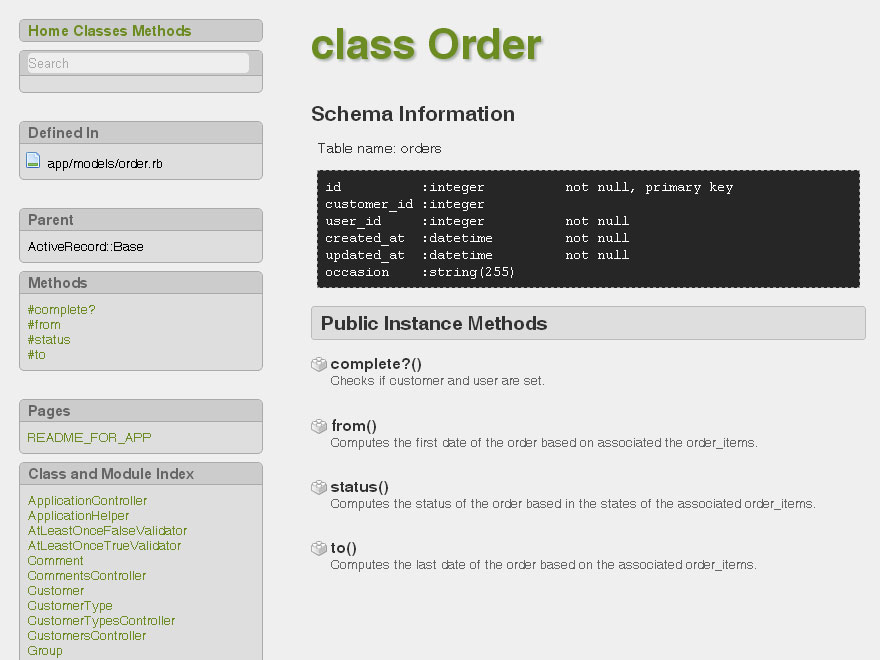
\includegraphics[width=\paperwidth]{images/rdoc}}
  \frame[plain]{}
}

\begin{frame}[fragile]{JSDoc}{public/app/models/order.js}
  \begin{lstlisting}[language=JavaScript,gobble=4]
    define(['backbone', 'app/models/base'],
        function (Backbone, ApplicationModel) {
      /**
       @class OrderModel
       @augments ApplicationModel
       */
      var OrderModel = ApplicationModel.extend(
      /**
       @lends OrderModel#
       */
      {
        /**
         * Name of this model.
         */
        name: 'order'
      });
      return OrderModel;
    });
  \end{lstlisting}
\end{frame}

\begin{frame}[fragile]{JSDoc}{lib/tasks/jsdoc.rake}
  \begin{lstlisting}[language=Ruby,gobble=4]
    namespace :doc do
      desc "Generate docs for the client."
      task :client do
        `jsdoc -r -d doc/client public/main.js public/app`
        puts "Created doc/client."
      end
    end
  \end{lstlisting}  
  
  \vskip3ex

  \begin{lstlisting}[language={},gobble=4]
    rake doc:client
  \end{lstlisting}
\end{frame}

{
  \setbeamertemplate{background canvas}{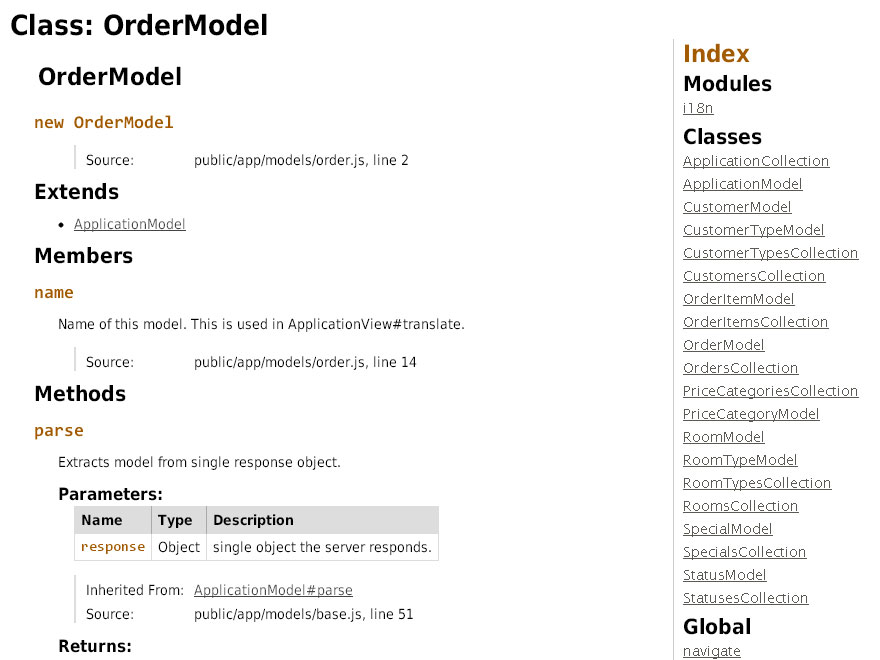
\includegraphics[width=\paperwidth]{images/jsdoc}}
  \frame[plain]{}
}